% small.tex
\documentclass{beamer}
\usetheme{Warsaw}

\usepackage[finnish]{babel}
\usepackage{lmodern}
\usepackage[utf8]{inputenc}
\usepackage[T1]{fontenc}
\usepackage{graphicx}

\title[Google Similarity Distance]{Google Samankaltaisuusetäisyys}
% \subtitle[Errors]{Estimation of numerical errors}
\author[T. Sand]{Timo Sand}
\institute[UH]{
  Tietojenkäsittelytieteen laitos\\
  Helsingin Yliopisto\\
  Helsinki\\[1ex]
}
\date[November 2013]{14. Marraskuu, 2013}

\begin{document}

\begin{frame}[plain]
  \titlepage
\end{frame}

\begin{frame}{Johdanto}
  The rise of the WWW has enticed millions of users to type in trillions of characters to create billions of Web pages of, on average, low-quality contents. The sheer mass of the information about almost every conceivable topic makes it likely that extremes will cancel and the majority or average is meaningful in a low-quality approximate sense. We devise a general method to tap the amorphous low-grade knowledge available for free on the WWW, typed in by local users aiming at personal gratification of diverse objectives, and, yet, globally achieving what is effectively the largest semantic electronic database in the world. Moreover, this database is available for all by using any search engine that can return aggregate page-count esti- mates for a large range of search-queries, like Google.
\end{frame}

\begin{frame}{Jäsentely}

\begin{itemize}
  \item Esimerkki
  \pause
  \item Algoritmin perusta
  \pause
  \item Samankaltaisuuden googlaus
  \pause
  \item Sovellukset ja kokeilut
  \pause
  \item Kertaus
\end{itemize}

\end{frame}

\begin{frame}{Esimerkki}
  At the time of doing the experiment, a Google search for “horse” returned 46,700,000 hits. The number of hits for the search term “rider” was 12,200,000. Searching for the pages where both “horse” and “rider” occur gave 2,630,000 hits, and Google indexed 8,058,044,651 Web pages. Using these numbers, we derive below, with $N = 8 058 044 651$, a Normalized Google Distance between the terms “horse” and “rider” as follows:
  \[
    NGD(horse, rider) \approx 0.443
  \]

    Values between 0 (identical) and 1 (unrelated)
\end{frame}

\begin{frame}{Algoritmin Perusta}
  The basis of much of the theory explored in this paper is Kolmogorov complexity.
    We assume a fixed reference universal programming system. Such a system may be a general computer language like LISP or Ruby, and it may also be a fixed reference universal Turing machine in a given standard enumeration of Turing machines.
    The Kolmogorov complexity of a string x is the length, in bits, of the shortest computer program of the fixed reference computing system that produces x as output. The Kolmogorov complexity K(x) gives a lower bound on the ultimate value: For every existing compressor, or compressors that are possible but not known, we have that K(x) is less than or equal to the length of the compressed version of x.
\end{frame}

\begin{frame}{Normalisoitu informaatioetäisyys}
  Given two strings x and y, what is the length of the shortest binary program in the reference universal computing system such that the program computes output y from input x, and also output x from input y? This is called the information distance and denoted as $E(x,y).$
  \[
    E(x, y) = K(x, y) - min{K(x), K(y)}
  \]
    $K(x,y)$ is the binary length of the shortest program that produces the pair x, y and a way to tell them apart.
    [We now consider a large class of admissible distances: All distances (not necessa- rily metric) that are nonnegative, symmetric, and computable in the sense that, for every such distance D there is a prefix program that, given two strings x and y, has binary length equal to the distance D(x, y) between x and y.]
    \[
      NID(x,y) =  K(x, y) - min(K(x), K(y)) / max(K(x), K(y))
    \]
\end{frame}

\begin{frame}{Normalisoitu pakkausetäisyys}
  The NID is uncomputable since the Kolmogorov complexity is uncomputable. But, we can use real data compression programs to approximate the Kolmogorov complexities. A compression algorithm defines a computable function from strings to the lengths of the compressed versions of those strings.
    Thus, if C is a compressor and we use C(x) to denote the length of the compressed version of a string x, then we arrive at the Normalized Compression Distance:
    \[
    NCD(x,y) =  C(xy) - min(C(x), C(y)) / max(C(x), C(y))
    \]
\end{frame}

\begin{frame}{Samankaltaisuuksien googlaus}
  The number of Web pages currently indexed by Google is approaching $10^10$. Every common search term occurs in millions of Web pages. This number is so vast, and the number of Web authors generating Web pages is so enormous (and can be assumed to be a truly representative very large sample from humankind), that the probabilities of Google search terms, conceived as the frequencies of page counts returned by Google divided by the number of pages indexed by Google, approximate the actual relative frequencies of those search terms as actually used in society.
\end{frame}

% \begin{frame}{Google-jakauma}
%   Let the set of singleton Google search terms be denoted by S. In the sequel, we use both singleton search terms and doubleton search terms $\{\{x,y\}:x,y e S\}$. Let the set of Web pages indexed (possibility of being returned) by Google be $\Omega$. The cardinality of $\Omega$ is denoted by $M = |\Omega|$

%     There are |S| singleton terms, and |S| over 2 doubletons consisting of a pair of nonidentical terms. Define $N = \Sum{\{x,y\}\subset S} |x \cap y|$. $N \geq M$
% \end{frame}
% \begin{frame}{Google samankaltaisuusetäisyys}
%   $NGD(x,y) = max\{log f(x),log f(y)\} - log f(x,y) / log N - min\{log f (x), log f (y)\}$
%     where f(x) denotes the number of pages containing x, and f (x, y) denotes the number of pages containing both x and y, as reported by Google.
% \end{frame}
\begin{frame}{Sovellukset: Hierarkinen klusterointi}
  \centering
  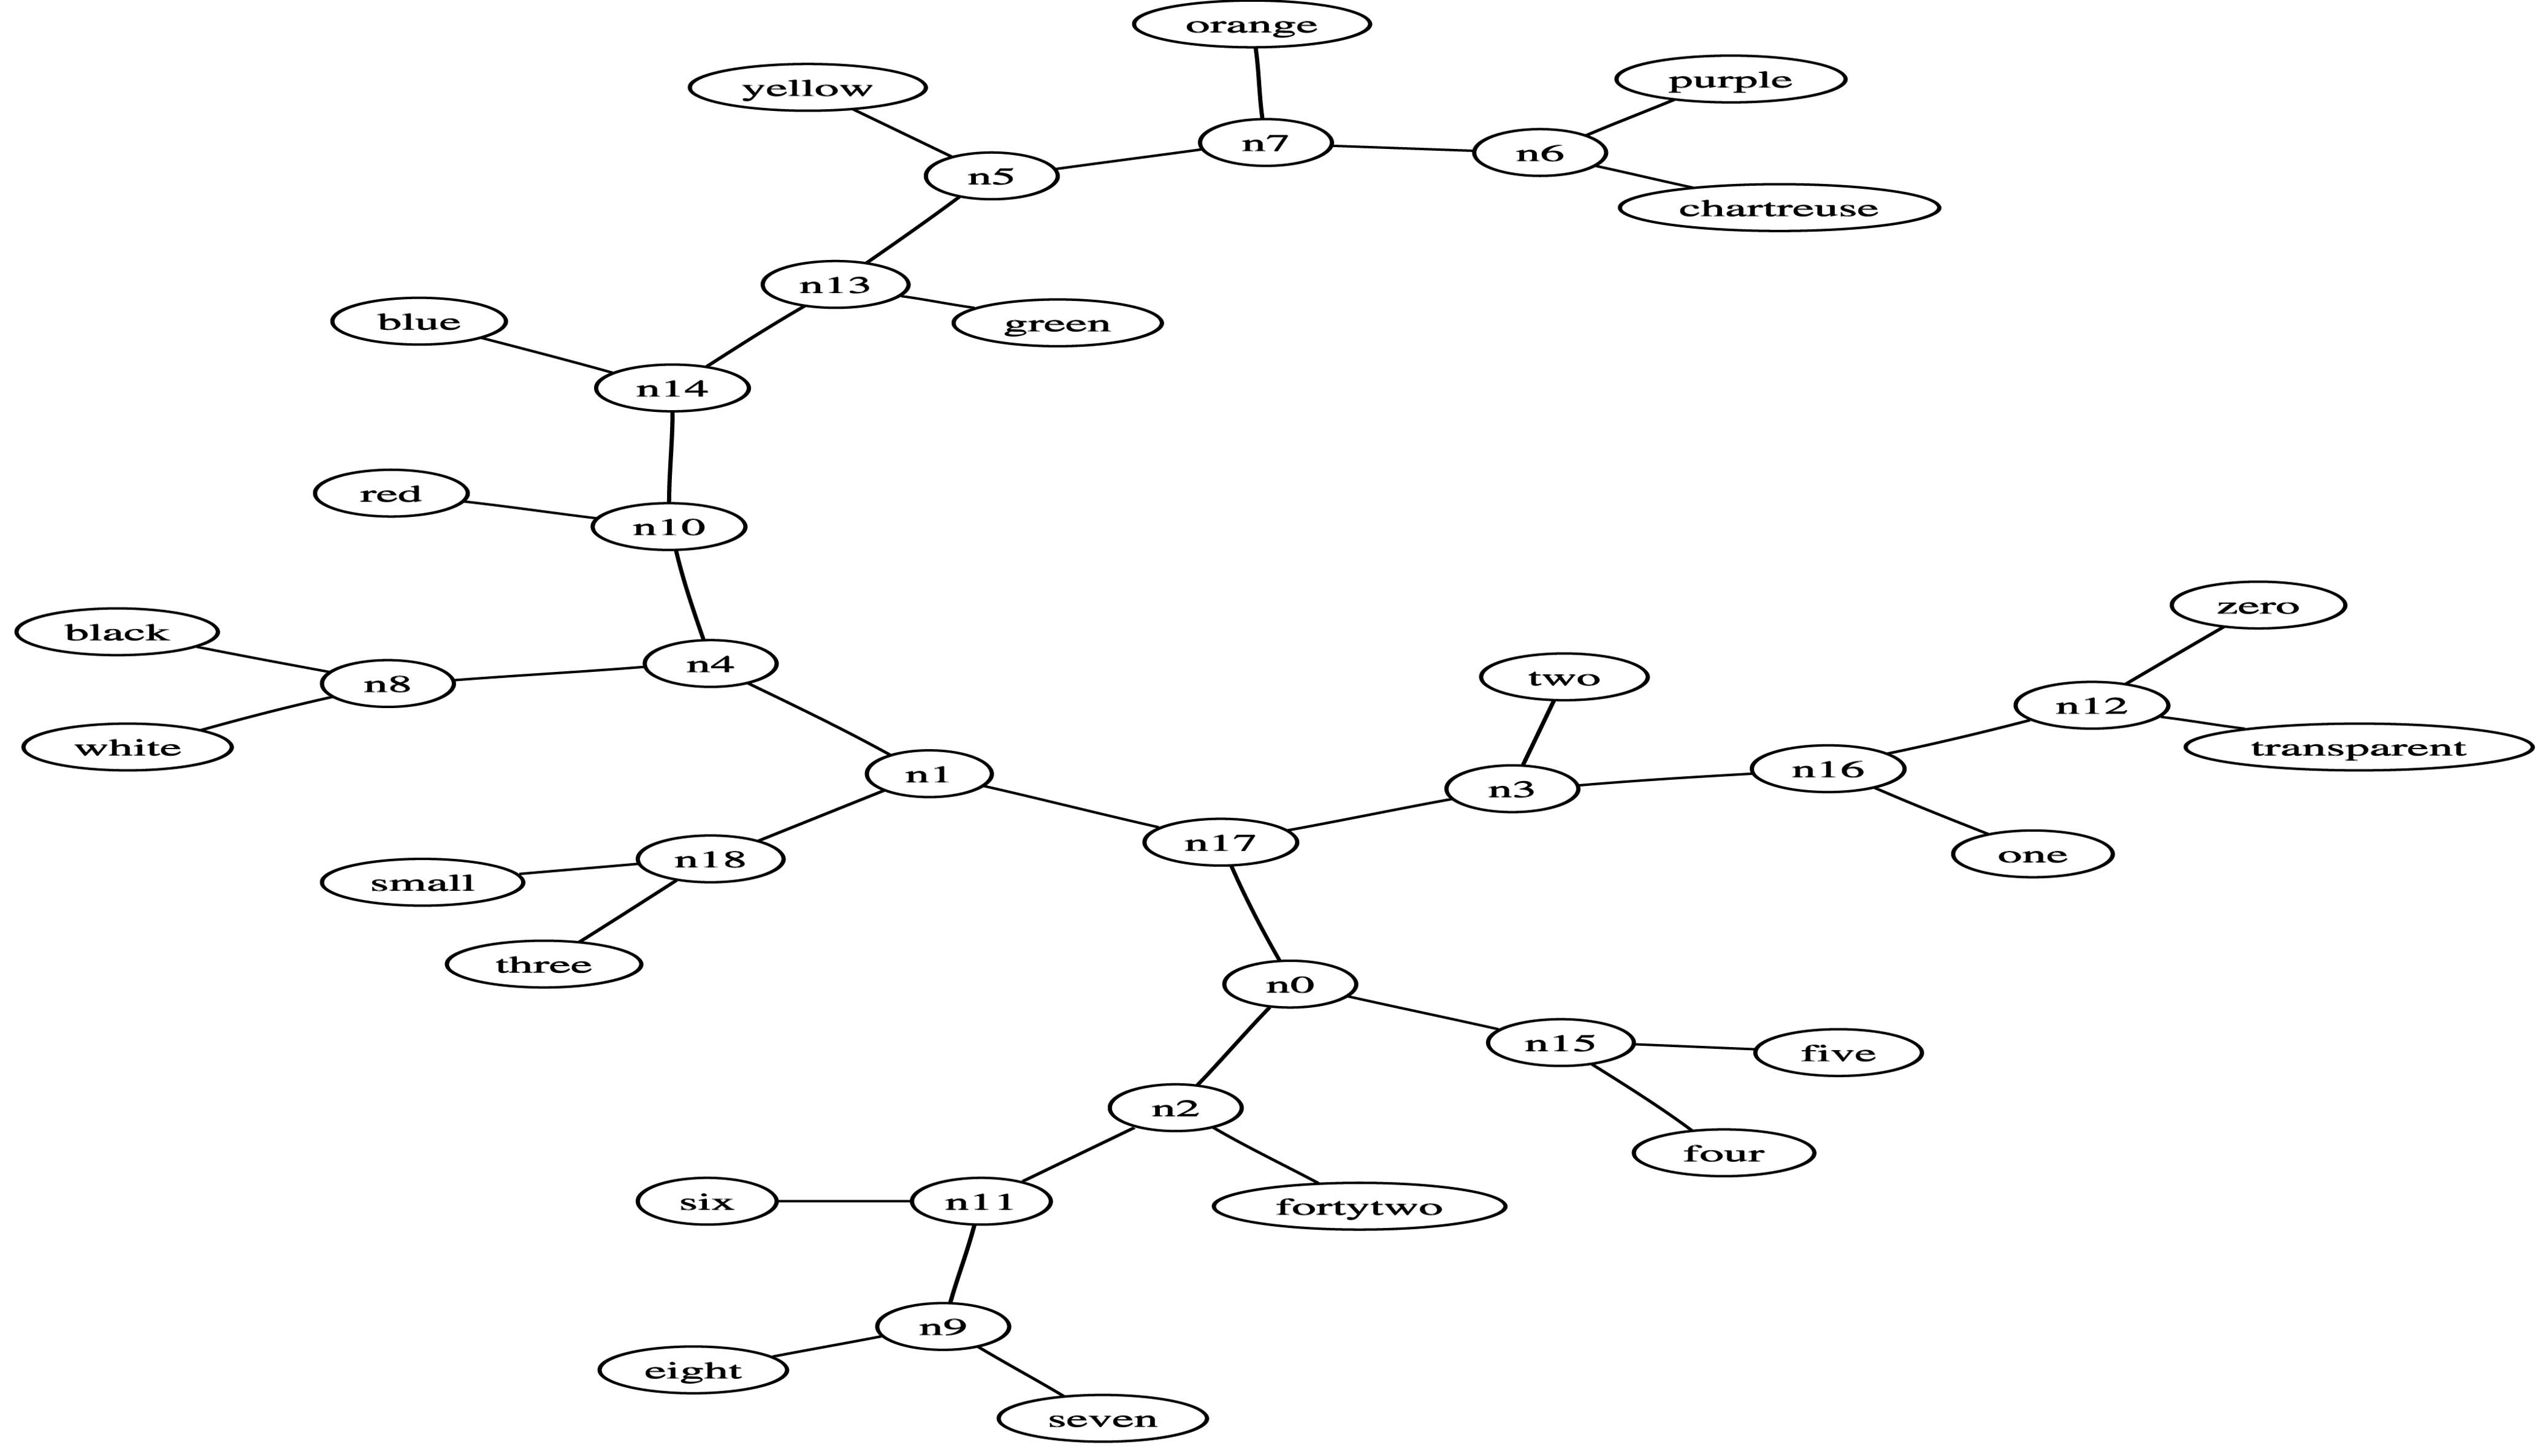
\includegraphics[width=8cm,keepaspectratio=true]{google-000}
\end{frame}

\begin{frame}{Sovellukset: Hollantilaisia maalareita}
  \centering
  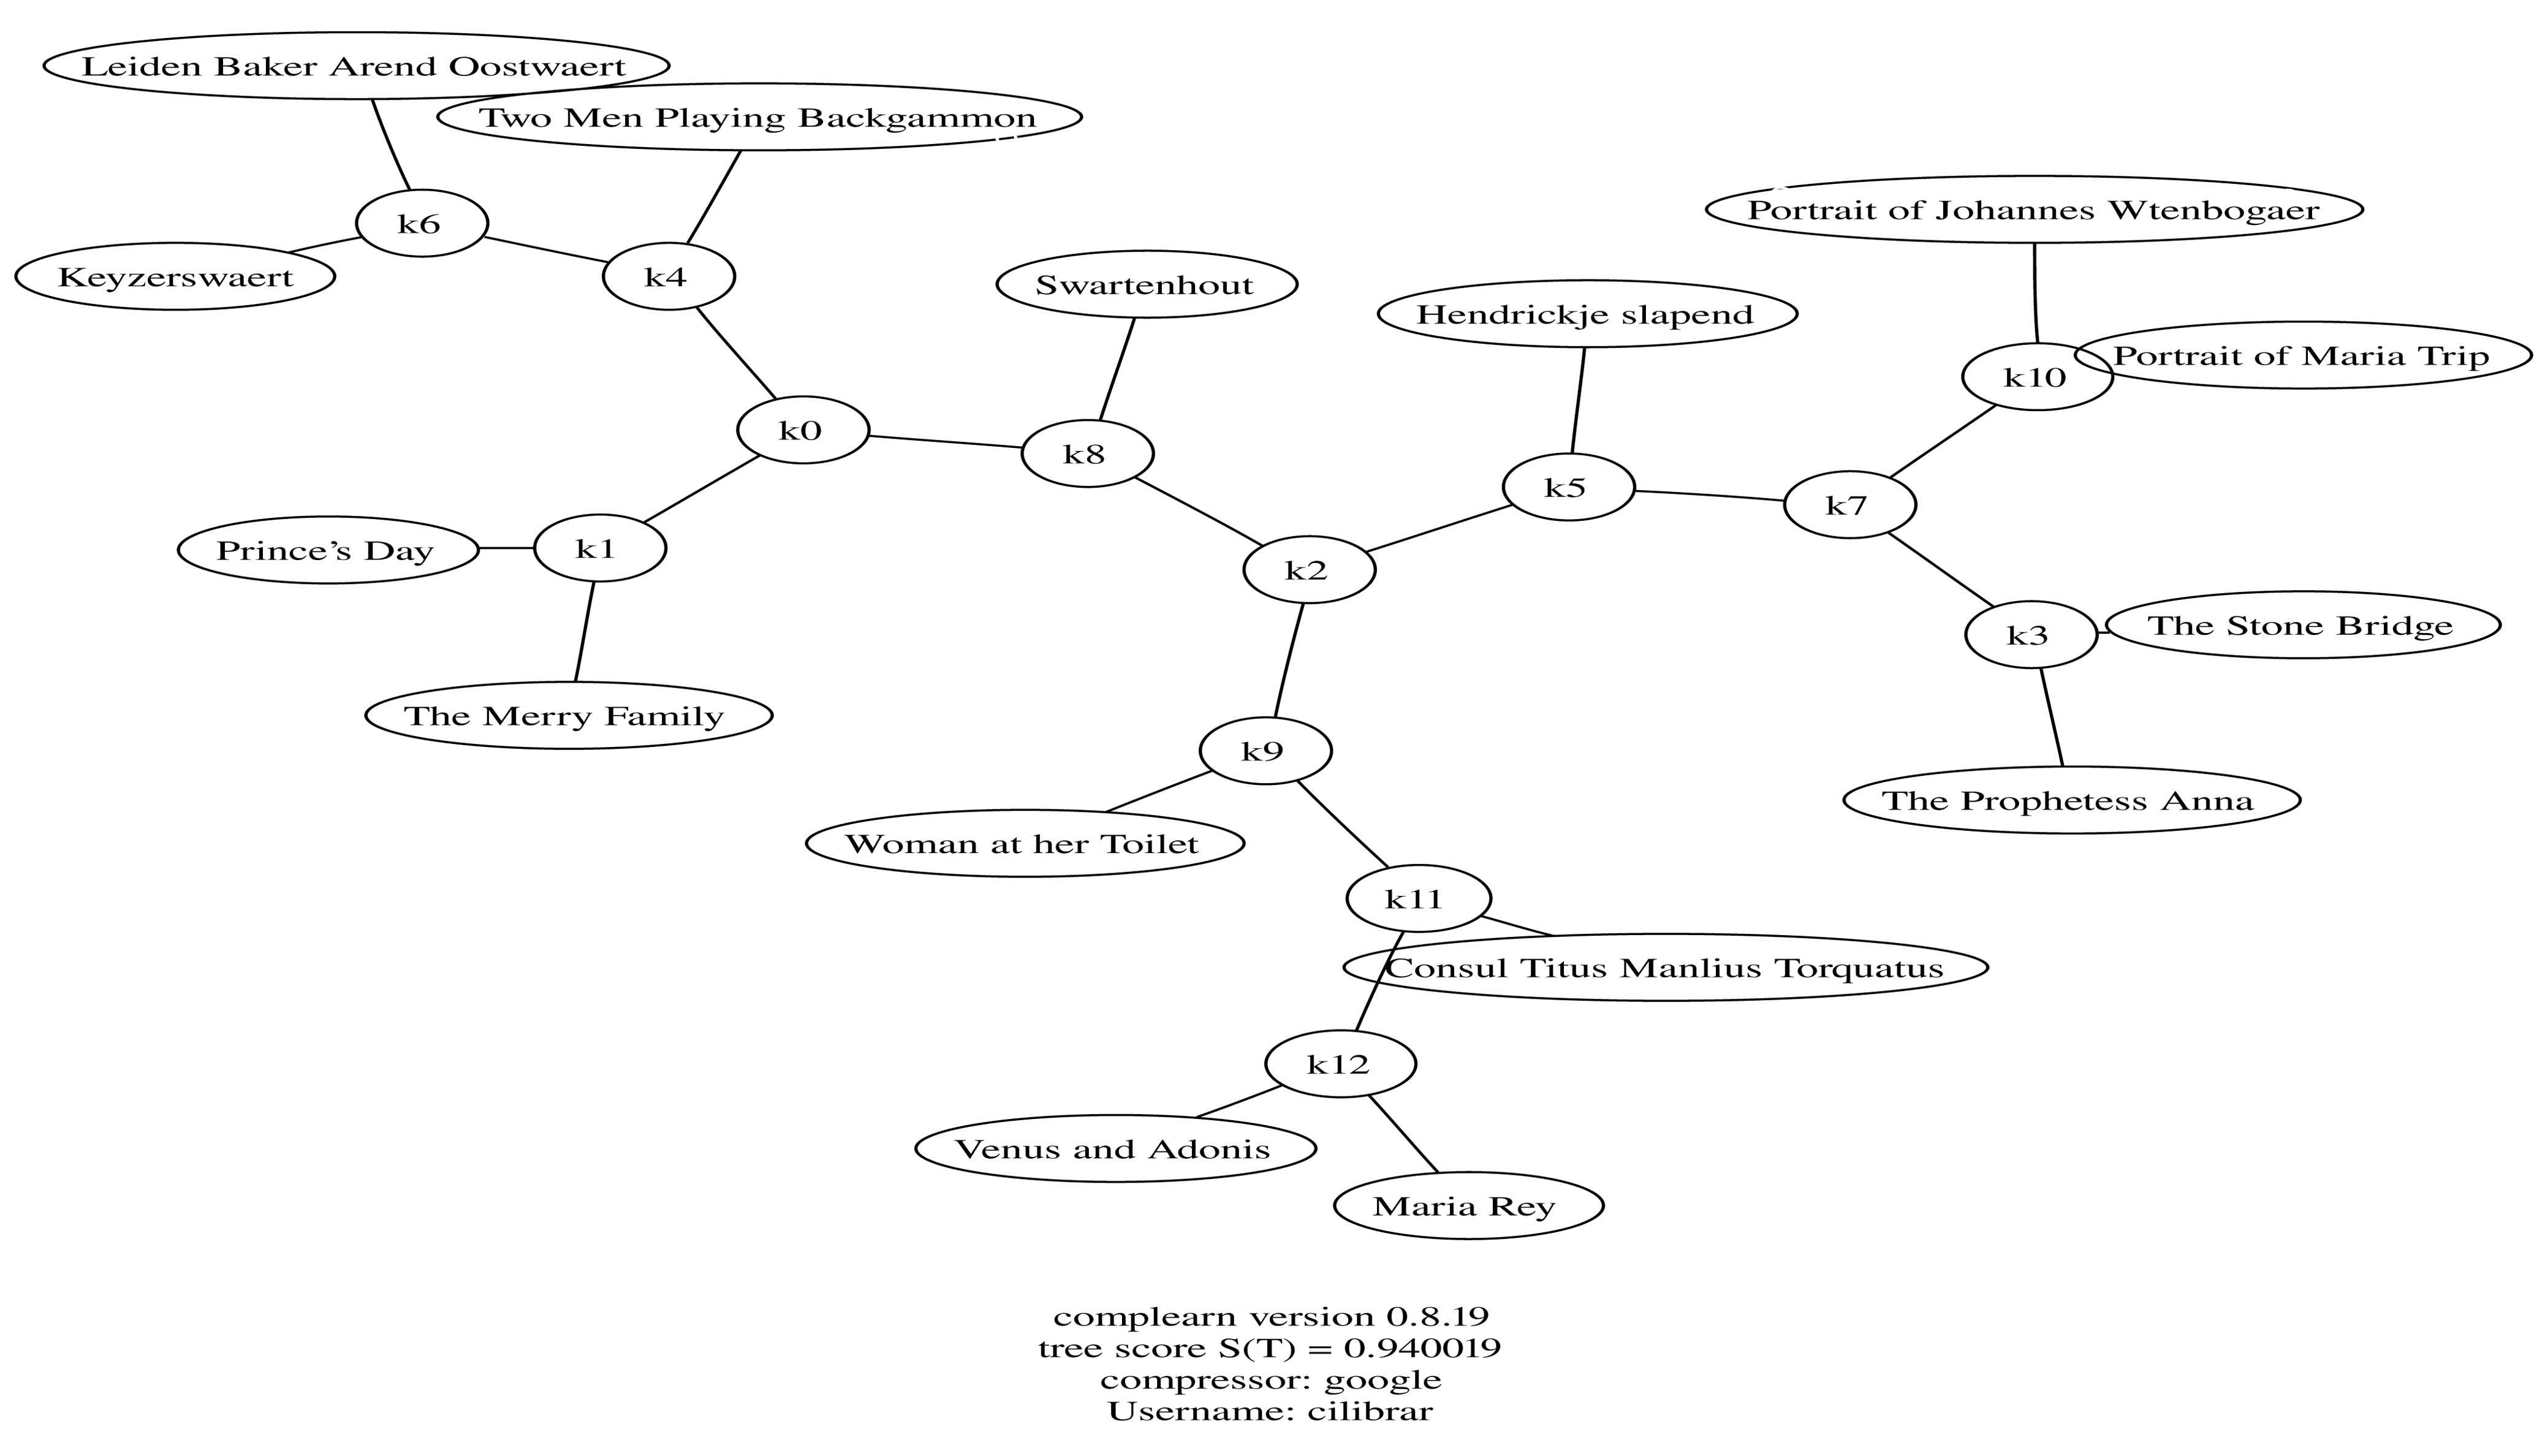
\includegraphics[width=8cm,keepaspectratio=true]{google-001}
\end{frame}

\begin{frame}{Sovellukset: Englantilaisia kirjailijoita}
  \centering
  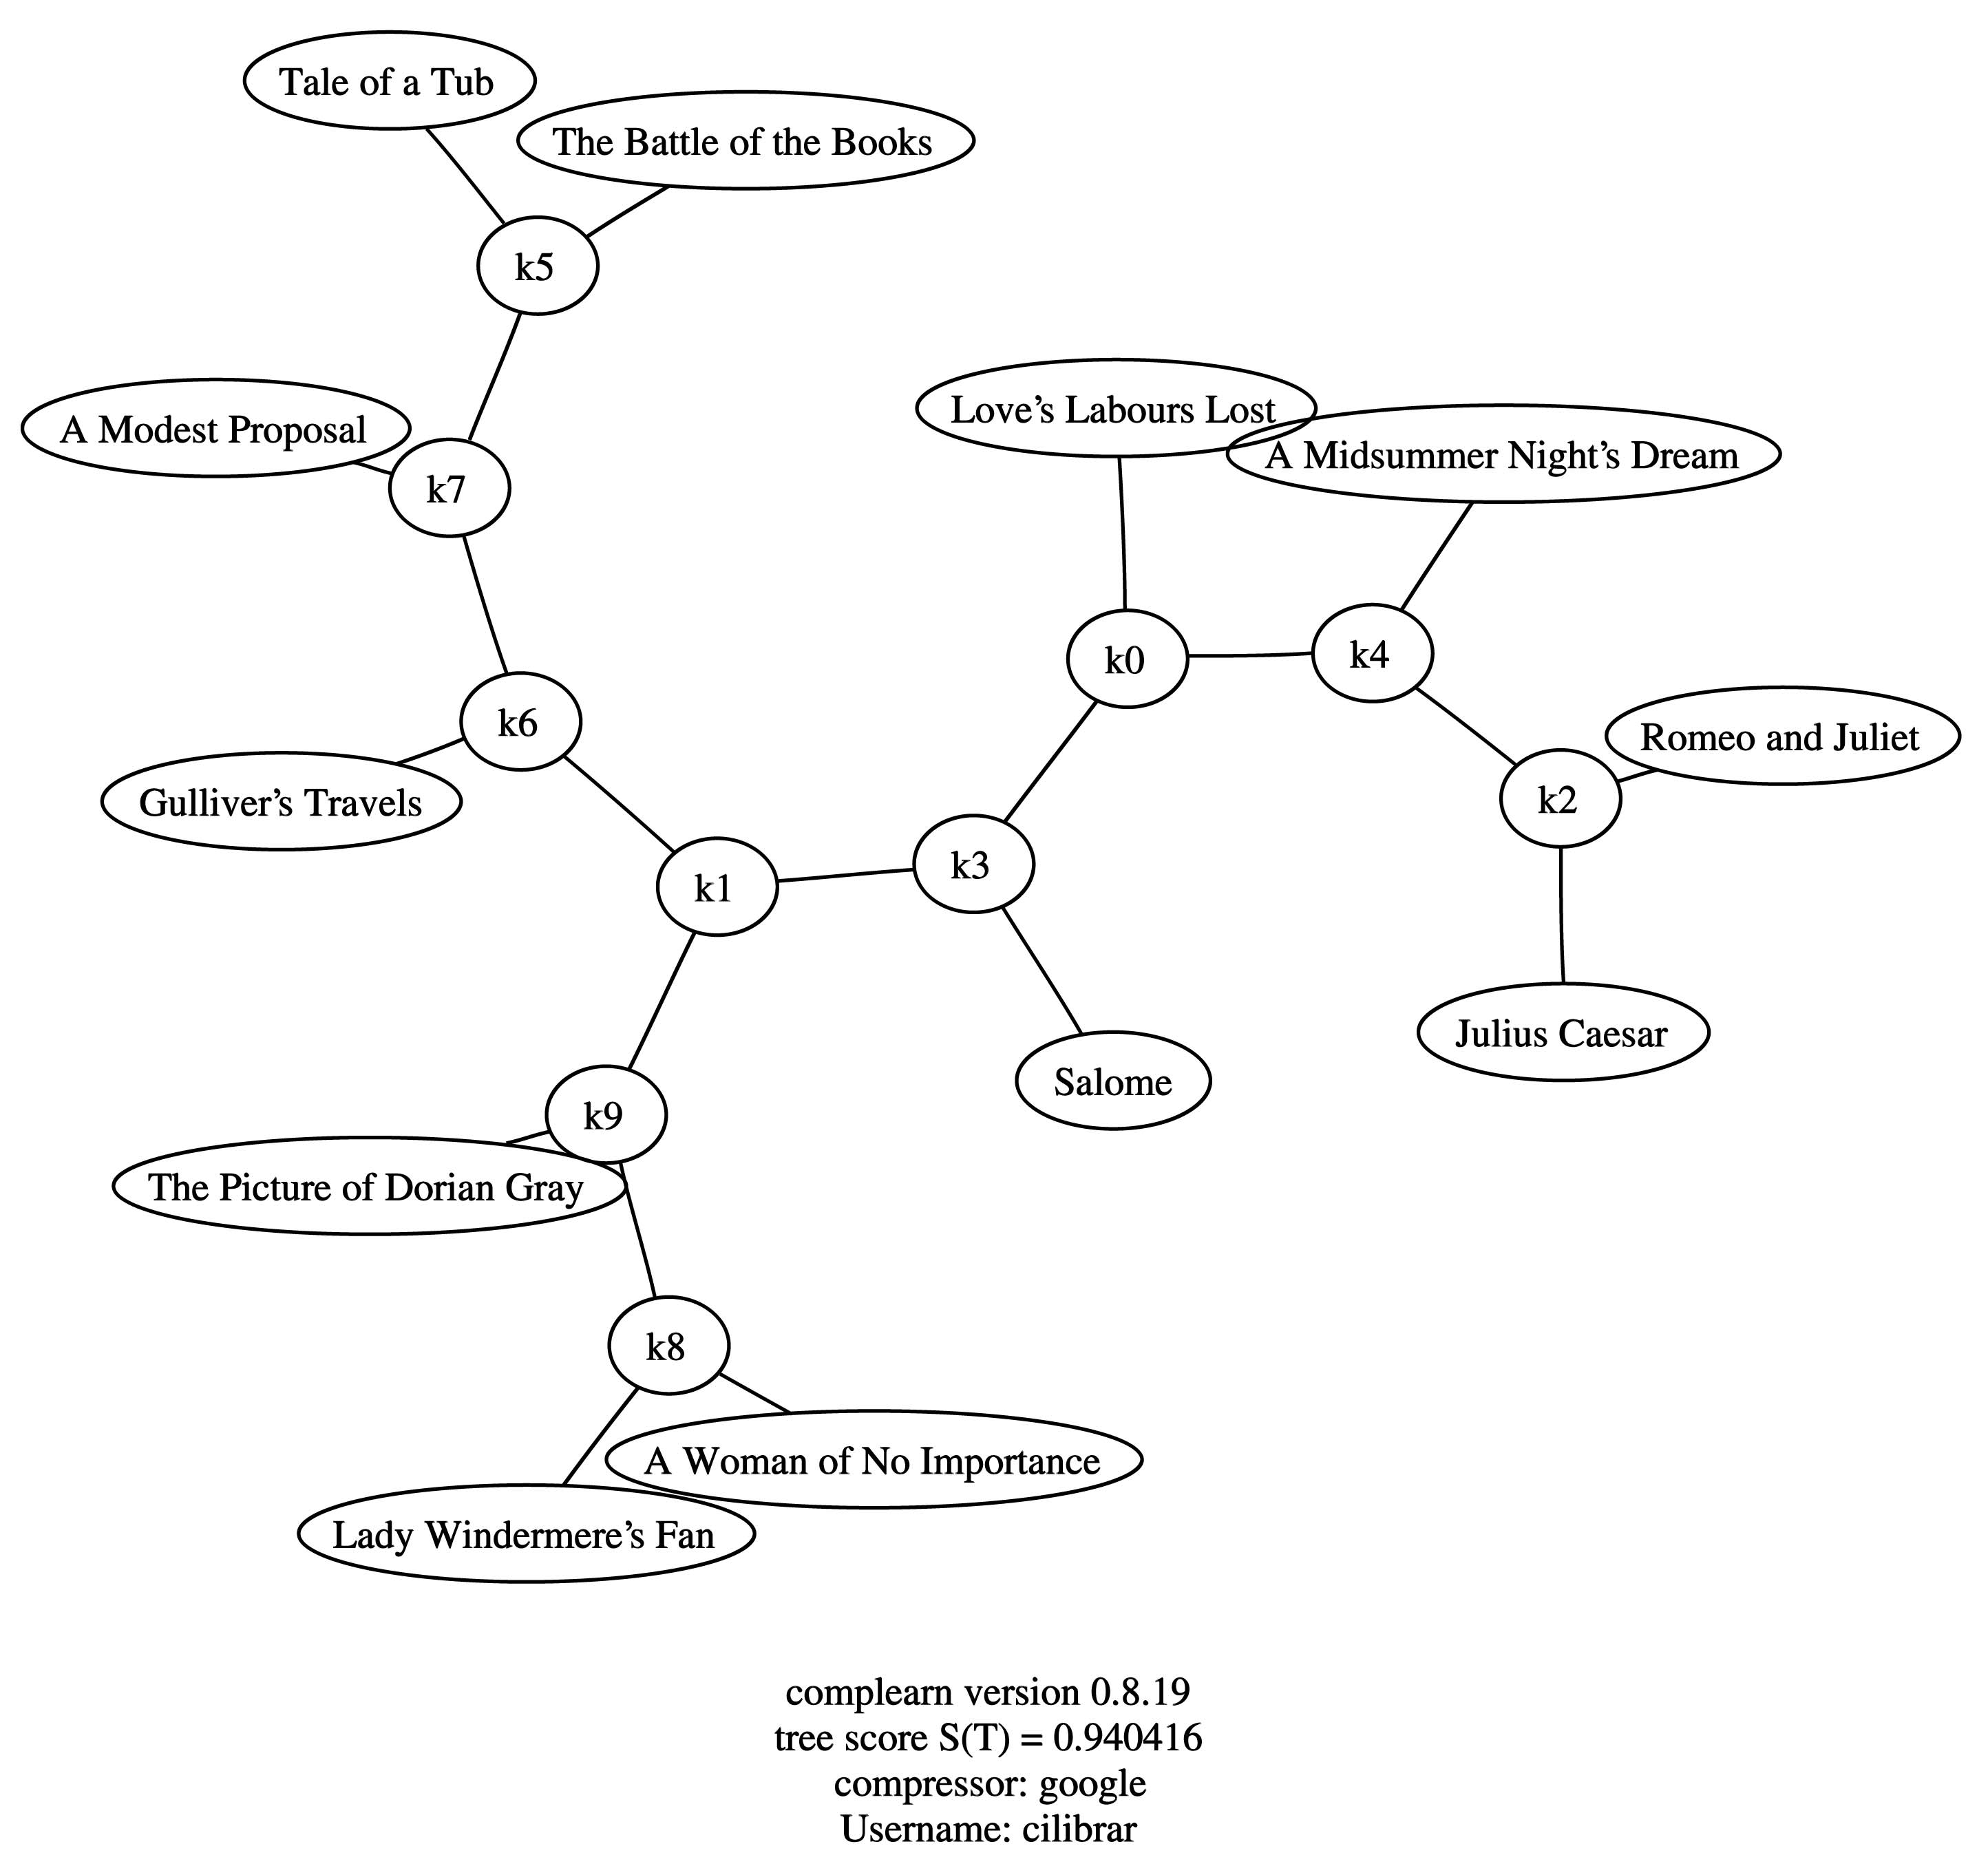
\includegraphics[width=8cm,keepaspectratio=true]{google-002}
\end{frame}

\begin{frame}{Kertaus}
  Kertaus
  \begin{itemize}
    \item NID
    \item NCD
    \item NGD
  \end{itemize}
\end{frame}

\begin{frame}
  \centering
  Kysymyksiä?
\end{frame}
\end{document}
